\documentclass[british]{article}
\usepackage[T1]{fontenc}
\usepackage{pdfpages}
\usepackage{fullpage}
\setlength{\parindent}{0em}
\setlength{\parskip}{1em}
\usepackage{setspace}
\onehalfspacing
\usepackage{babel}
\usepackage{csquotes}
\SetBlockThreshold{2}
\usepackage{graphicx}
\DeclareGraphicsExtensions{.jpg,.png}
\graphicspath{{./images/}}
\usepackage{float}
\usepackage{url}
\usepackage{listings}
\lstset{escapeinside={<@}{@>}}
\usepackage{color}

\title{PG6300-14 Webutvikling \& API-design lecture notes 09: Testing}
\author{Martin Lehmann}
\date{\today}

\begin{document}

\maketitle

\section{Intro}
Core functionality is now complete (except security in WebSockets -- not part of the curriculum.

Stability time! Testing is a great way of ensuring stability AND expressing user stories (thus removing the need for extensive documentation).

Tests developers know when they made a mistake that messed up the rest of the application. You've all done (part of) this before.

A well-written application uses both end-to-end and unit tests on both the client and the server.

Minor side note: \textbf{Dev dependencies}

\begin{lstlisting}
$ npm install --save mongoose
$ npm install --save-dev gulp
\end{lstlisting}

\section{End-to-end testing}

\begin{itemize}
  \item Test \textit{everything} from UI to database
  \item Slow, but very good for catching errors (catch everything)
\end{itemize}

\subsection{Protractor}

\begin{itemize}
  \item A tool for running end-to-end tests in Angular JS applications
  \item Not limited to Angular, but specifically designed for Angular (by the AngularJS team)
  \item Protractor is a Node.js app
  \item Uses WebDriver \& Selenium to run an actual browser (thus, slow)
  \item Intall as dev dependency via NPM
    \begin{lstlisting}
$ npm install --save-dev protractor        
    \end{lstlisting}
  \begin{itemize}
      \item Protractor has very large files for an NPM package -- don't include it as a production dependency as deployment will be slowed down.
  \end{itemize}
  \item Set up WebDriver with Selenium "automagically"
    \begin{lstlisting}
$ ./node_modules/.bin/webdriver-manager update
Updating selenium standalone
downloading https://selenium-release.storage.googleapis.com/2.45/selenium-server-standalone-2.45.0.jar...
Updating chromedriver
downloading https://chromedriver.storage.googleapis.com/2.14/chromedriver_mac32.zip...
chromedriver_2.14.zip downloaded to /Users/theneva/Dropbox/WACT/PG6300 Webutvikling og API-design/f09-testing/first-end-to-end-project/node_modules/protractor/selenium/chromedriver_2.14.zip
selenium-server-standalone-2.45.0.jar downloaded to /Users/theneva/Dropbox/WACT/PG6300 Webutvikling og API-design/f09-testing/first-end-to-end-project/node_modules/protractor/selenium/selenium-server-standalone-2.45.0.jar
$ 
    \end{lstlisting}
  \item Protractor is just a test \textit{runner}. Time to add a testing framework!
  \item Several options
  \begin{itemize}
    \item QUnit (for JQuery): inflexible, verbose, weak when it comes to asynchronous and promise-based testing
    \item Jasmine (for Behavious-Driven Development): Based on testing in Ruby. Much more concise than QUnit, but weak when it comes to asynchronous and promise-based testing. The choice for most Angular apps (including the Angular team)
    \item Mocha: The choice for most Node applications. Flexible, pick \& choose tools that fit your application. Well supported with all Angular tools. Will be using this.
  \end{itemize}
\end{itemize}

\subsection{Mocha}
\begin{itemize}
  \item Test framework (you write tests with Mocha, just like with JUnit for Java, NUnit for .NET, XCTest for Objective-C and Swift, and so on
  \item Requires a few configuration options, but nothing too bad
\end{itemize}

\subsection{Basic Protractor test}
\begin{itemize}
  \item Convention to put all tests in \textit{project root}/test/
  \item Three different test methods:
  \begin{itemize}
    \item End-to-end: \textit{project}/test/e2e/
    \item Node server: \textit{project}/test/node
    \item Angular: \textit{project}/test/angular
    \item ex:
      \begin{lstlisting}
$ mkdir -p test/e2e test/angular test/node

project root
`- test
  `- angular
  `- e2e
  `- node
      \end{lstlisting}
  \end{itemize}
\end{itemize}

\subsubsection{First test time!}
\begin{itemize}
  \item Protractor is great for describing user stories; design tests with users in mind
  \item E-commerce: Come to the site, find a product, add it to the shopping card, complete the order
  \item Tests hit many (all?) parts of the application and ensure that common flows are always stable
  \item Too many tests (or too fine-grained tests) become too slow, take too long to write, and thus changing design becomes bad. Feature tests are good, but use with care
\end{itemize}

First test: test/e2e/making-a-post.spec.js
\begin{lstlisting}
describe('making a post', function() {
    it('logs in and creates a new post', function() {
        // go to homepage
        // click 'login'
        // fill out and submit login form
        // submit a new post on the posts page
        
        // The new post should be visible as the first post on the page
    });
});
\end{lstlisting}

\begin{itemize}
  \item Tests MUST be named *.spec.js for Protractor to find them -- this allows us to have normal .js utility files that are not treated as tests
  \item "descibe" describes a test scenario to give context. Can be nested!
  \item "it" is an actual test
  \item Final assertion on its own line ('The new post should be visible as the first post on the page'): Think of the final assertion first. What should ultimately be tested? Could describe the flow backwards so that you only need to think of one prerequisite at a time.
\end{itemize}

From pseudocode to a (barely) running test (test/e2e/making-a-post.spec.js):
\begin{lstlisting}
describe('making a post', function() {
    it('logs in and creates a new post', function() {
        // go to homepage
        browser.get('http://localhost:3000');
        // click 'login'
        // fill out and submit login form
        // submit a new post on the posts page
        
        // The new post should be visible as the first post on the page
    });
});
\end{lstlisting}

Configure Protractor to use Mocha (and tell it where to find your tests)

\textit{project root}/protractor.conf.js
\begin{lstlisting}
exports.config = {
    framework: 'mocha',
    specs: [
        'test/e2e/**/*.spec.js'
    ]
};
\end{lstlisting}

Install Mocha as a dev dependency:

\begin{lstlisting}
$ npm install --save-dev mocha
\end{lstlisting}

Run Protractor (the same command as previously, but without 'update'). \textbf{NB}: This requires the file retrieved at \url{http://localhost:3000} to be an actual Angular application. You cannot run this on an empty HTML file!

\begin{lstlisting}
$ ./node_modules/.bin/protractor    
\end{lstlisting}

This...
\begin{itemize}
  \item Opens a browser window briefly (that's WebDriver/Selenium, required to actually perform the tests)
  \item Prints information in the console:
\end{itemize}

\begin{lstlisting}
./node_modules/.bin/protractor
Starting selenium standalone server...
[launcher] Running 1 instances of WebDriver
Selenium standalone server started at http://10.21.24.41:64200/wd/hub

  <@\textcolor{green}{.}@> making a post logs in and creates a new post: <@\textcolor{red}{457ms}@>

  <@\textcolor{green}{1 passing}@> (460ms)

Shutting down selenium standalone server.
[launcher] 0 instance(s) of WebDriver still running
[launcher] chrome #1 passed    
\end{lstlisting}

Start node inside Protractor to avoid having to keep the server running at all times.

\textit{project root}/protractor.conf.js
\begin{lstlisting}
exports.config = {
    framework: 'mocha',
    specs: [
        'test/e2e/**/*.spec.js'
    ],
    <@\textcolor{blue}{onPrepare}@>: function() {
        require('./server-node/hello-tests-server.js');
    }
};
\end{lstlisting}

\dots but this makes you unable to already have a server running. Use a different port set by environment variables!

Edit server.js to pick its port from an environment variable:

\begin{lstlisting}
var express = require('express');
var app = express();
<@ \dots @>
var port = <@\textcolor{blue}{process.env.PORT ||}@> 3000;
<@ \dots @>
app.listen(port, function() {
    console.log('Listening on port ' + port);
});
\end{lstlisting}

Then set the environment variable inside Protractor's onPrepare:

\textit{project root}/protractor.conf.js

\begin{lstlisting}
exports.config = {
    framework: 'mocha',
    specs: [
        'test/e2e/**/*.spec.js'
    ],
    onPrepare: function() {
        <@\textcolor{blue}{process.env.PORT = 3001;}@>
        require('./server-node/hello-tests-server.js');
    }
};
\end{lstlisting}

\dots and finally point the test code to the port of the server started by Protractor (3001):

\begin{lstlisting}
describe('making a post', function() {
        it('logs in and creates a new post', function() {
                // go to homepage
                browser.get('http://localhost:<@\textcolor{blue}{3001}@>');
                // click 'login'
                // fill out and submit login form
                // submit a new post on the posts page

                // the new post should be visible as the first post on the page
        });
});
\end{lstlisting}

Protractor \textbf{Locators}

Interact with the DOM elements on the page! For more information, see \url{https://github.com/angular/protractor/blob/master/docs/locators.md}.

First, get a hold of the DOM element:

\begin{lstlisting}
// find an element using css selector
by.css('.someclass');

// find an element using id
by.id('someid');

// find an element by ng-model (e.g. username)
by.model('username');

// find an element by binding (e.g., {{currentUser}})
by.binding('currentUser');

// find an element by repeater (e.g., item in items
by.repeater('item in items');
\end{lstlisting}

Pass the locator to element(locator), and you can interact with it:

\begin{lstlisting}
// click a button or link
element(by.css('.mybutton')).click();

// fill out a text input
element(by.css('.username-input')).sendKeys('theneva');
\end{lstlisting}

\textbf{NB}: These are all asynchronous events!

Now to actually write a test, add the class 'login' to the Login link in the navbar:

\begin{lstlisting}
<a class="navbar-text navbar-right <@\textcolor{blue}{login}@>" href="/#/login" ng-if="!currentUser">Log in</a>
\end{lstlisting}

Then use Protractor locators to select and click the link:

\begin{lstlisting}
// click 'login'
var loginLink = element(by.css('nav .login'));
loginLink.click();    
\end{lstlisting}

\textbf{NB}: Entering a nonexistent ID results in a failed test.

Now fill in the login form, click the login button, and save a new item:

\begin{lstlisting}
// fill out and submit login form
var usernameInput = element(by.model('username'));
usernameInput.sendKeys('theneva');

var passwordInput = element(by.model('password'));
passwordInput.sendKeys('1234');

// Click the login button
var loginButton = element(by.css('.button-login'));
loginButton.click();

// save a new item on the home page
var nameInput = element(by.model('newItem.name'));
nameInput.sendKeys('Some random item');

var saveButton = element(by.css('.button-save'));
saveButton.click();
\end{lstlisting}

Now get a hold of the the item on top of the list so we are ready to make our assertion that the new item was added to the top:

\begin{lstlisting}
// the new item should be visible as the first item on the page
element.all(by.repeater('item in items')).then(function(items) {
	var firstItem = items[0];
	firstItem.element(by.css('.item-name')).getText().then(function(firstItemName) {
		console.log(firstItemName);
	});

	firstItem.element(by.css('.item-author')).getText().then(function(firstItemAuthor) {
		console.log(firstItemAuthor);
	});
});
\end{lstlisting}

Finally, to make our assertions, we need an assertion library: chai. Install as a dev-dependency with NPM:

\begin{lstlisting}
$ npm install --save-dev chai
\end{lstlisting}

Require the appropriate function and make assertions in test/make-an-item.spec.js:

\begin{lstlisting}
var expect = require('chai').expect;
\dots
firstItem.element(by.css('.item-name')).getText().then(function(firstItemName) {
	<@\textcolor{blue}{expect(firstItemName).to.equal(itemContent);}@>
});

firstItem.element(by.css('.item-author')).getText().then(function(firstItemAuthor) {
	<@\textcolor{blue}{expect(firstItemAuthor).to.equal(username);}@>
});
\end{lstlisting}

If the returned content was wrong (e.g. the logged in user's username was 'hello', but the author of the post still showed as 'theneva', you would see message in \ref{fig:wrong-assertion}.

\begin{figure}[H]
    \label{fig:wrong-assertion}
    \centerline{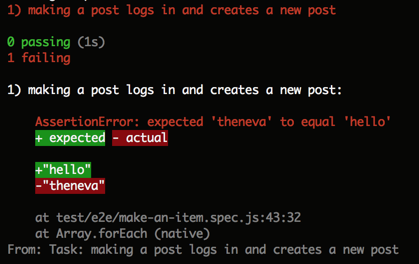
\includegraphics[scale=0.7]{wrong-assertion}}
    \caption{Wrong assertion}
\end{figure}

\textit{browser.pause()} in your tests is a nice tool that lets you pause the test execution and step through so you can see exactly what happens.

The current test stack is as follows: \textbf{Protractor} sets up \textbf{Selenium} and \textbf{WebDriver} and spins up a separate instance of the server on port 3001,  before running all tests in \textit{project root}/test/e2e/ using the testing framework \textbf{Mocha}, which in turn uses \textbf{Chai} to make assertions.

A final trick for end-to-end testing can help avoid that the tests get messy. This can be avoided with the NPM package chai-as-promised, but we will not be looking into this in detail.

One key thing to note is that we are working directly with the application's database. Clearing out the test data is probably a good idea, but figuring out a good way to do it requires some thought. A very simple way to deal with this is simply dropping the database with a Protractor afterEach filter, which works just like onPrepare – simply require the database file (which exports the connected Mongoose instance) and run \textit{the-module}.connection.db.dropDatabase();

If you only have time and resources to test one aspect of your application, then end-to-end tests are probably the absolutely most important kind of tests to write. They use the application like a user is expected to use it, and will be a major player in preventing bugs that directly affect the end users.

\section{Unit testing}

\begin{itemize}
  \item Test isolated components (single units, also known as functions and classes)
  \item Used in both Node and Angular, but completely separately
  \item Every test is ignorant of the other tests
  \item These are the tests you write before coding
  \item Great for test-driven development (TDD)
\end{itemize}

\end{document}